\documentclass[a4paper,12pt,oneside,onecolumn]{uerj}

\usepackage[brazil]{babel}  % adequacao para o portugues Brasil
\usepackage{cmap}           % Mapear caracteres especiais no PDF
\usepackage[utf8]{inputenc} % Determina a codificacao utiizada
                            % (conversão automática dos acentos)
\usepackage{listings}
\usepackage{makeidx}        % Cria o indice
\usepackage{hyperref}       % Controla a formacao do indice
\usepackage{indentfirst}    % Indenta o primeiro paragrafo de cada secao.
\usepackage{color}          % Controle das cores
\usepackage{graphicx}       % Inclusao de graficos
\usepackage{amsmath,amssymb}        % pacote matemático
\usepackage{pdfpages}
\usepackage[top=3cm, bottom=2cm, left=3cm, right=2cm]{geometry}

\usepackage[frame=no,gride=no,algline=yes,font=default]{uerjformat}
\usepackage[alf]{abntcite}
\newcommand{\formato}[1]{\begin{flushleft}{#1}\end{flushleft}}
\newcommand{\BibTeX}{{{Bib}}\TeX}

\logo{uerj/logo_uerj_cinza.png}
\marcadagua{uerj/marcadagua_uerj_cinza.png}{1}{160}{255}


\instituicao{Universidade do Estado do Rio de Janeiro}
            {Centro de Tecnologia e Ciências}
            {Instituto de Matemática e Estatística}
            {Departamento de Informática e Ciência da Computação}

\autor{Juan}{Lopes}
\titulo{Uma Implementação de Expressões Regulares em Tempo Polinomial}

\orientador{Prof.} % rotulo
           {Paulo Eustáquio Duarte}{Pinto, DSc.} % {nome}{sobrenome}
           {} % afiliacao

\coorientador{titulação} % rotulo
           {[nome de]}{[sobrenome]} % {nome}{sobrenome}
           {[afiliação]} % afiliacao


\grau{Bacharel}
\curso{Informática e Tecnologia da Informação}

\local{Rio de Janeiro}   % cidade
\data{17}{Maio}{2013} % {dia}{mes}{ano}

% *****************************************************************************
% *****************************************************************************
% Configurações de aparência do PDF final
% *****************************************************************************
% *****************************************************************************

% alterando o aspecto da cor azul
%\definecolor{blue}{RGB}{41,5,195}

% informações do PDF
\hypersetup{
  %backref=true,
  %pagebackref=true,
  %bookmarks=true,                  % show bookmarks bar?
  pdftitle={\UERJtitulo},
  pdfauthor={\UERJautor},
  pdfsubject={\UERJpreambulo},
  pdfkeywords={Expressões Regulares}{Regex}{Autômatos Finitos},
  pdfproducer={LaTeX with class repUERJ}, % producer of the document
  pdfcreator={\UERJautor},
  colorlinks=true,                  % false: boxed links; true: colored links
  linkcolor=black,                   % color of internal links blue
  citecolor=black,                    % color of links to bibliography blue
  filecolor=black,                % color of file links magenta
  urlcolor=black,
  bookmarksdepth=4
}


\makeindex

\begin{document}

\frontmatter
\capa
\folhaderosto

%\includepdf{ficha_catalografica.pdf}

\begin{folhadeaprovacao}
  \assinatura{titulação membro1\\ afiliação1}
\end{folhadeaprovacao}

\pretextualchapter{Dedicatória}

  \vfill\vfill
    \hfill À minha esposa, Jacqueline.
  \vfill


\pretextualchapter{}

  \vfill\vfill\vfill\vfill
  \begin{flushright}
     Simplicity is a great virtue but it requires hard work\\
     to achieve it and education to appreciate it. And to \\
     make matters worse: complexity sells better.\\
    \textsl{-- Edsger W. Dijkstra}
  \end{flushright}
  \vfill

% ----------------------------------------------------------
% RESUMO
% ----------------------------------------------------------

\pretextualchapter{Resumo}

\refbibliografica

Na teoria, expressões regulares constituem uma notação para definir linguagens regulares em termos de operações recursivas simples. São equivalentes a autômatos finitos em seu poder expressivo. Na prática entretanto, enquanto ferramentas extremamente populares, as expressões regulares modernas afastaram-se bastante da teoria que as originou. 

A maior parte das mudanças aconteceu para permiti-las alcançar um poder de expressão maior. Entretanto, esta conveniência veio a custo de tornar o \emph{match} um problema mais difícil computacionalmente do que a teoria descreve. Na maior parte das linguagens modernas o \emph{match} de \emph{regexes} (como são comumente conhecidas) é um problema NP-completo. Além disso, por particularidades de como são implementadas, mesmo expressões que poderiam ser reconhecidas em tempo polinomial são resolvidas com soluções exponenciais. 

Este trabalho visa analisar as armadilhas comuns no desenvolvimento de expressões regulares, realizando benchmarks entre diversas implementações populares, apontando funcionalidades que impediriam sua execução polinomial. Também sugere uma implementação simples e didática que tem desempenho em pior caso ordens de grandeza superior às bibliotecas-padrão de muitas linguagens.

\noindent {Palavras-chave}: Teoria da computação. Expressões regulares. Linguagens regulares. Autômatos finitos. Complexidade computacional. Algoritmos. NP-completo.

% ----------------------------------------------------------
% Abstract
% ----------------------------------------------------------

\pretextualchapter{Abstract}

In theory, regular expressions are a notation to define regular languages in terms of simple recursive operations. Are equivalent to finite automata in its expressive power. In practice however, while very popular tools, modern regular expressions did deviate from the theory that gave them origin.

Most of the changes happened to allow them to reach a greater expressive power. This convenience, however came at the cost of making the match a computationally harder problem than what theory describes. In most of the modern languages, the regex match (as it is commonly known) is a NP-complete problem. Besides, the way they are implemented makes even expressions that could be recognized in polynomial time to be solved with exponential algorithms.

This work aims to analyze the common pitfalls in regular expressions development, measuring performance with benchmarks of the most popular implementations, pointing the features that could not be implemented in polynomial time. Also it suggests a simple and didactic implementation which has superior worst-case performance than many language's standard libraries.

\noindent {Keywords}: Computation theory. Regular expressions. Regular languages. Finite automata. Computational complexity. Algorithms. NP-complete.

\listadefiguras
%\listadetabelas

\sumario

\mainmatter

%======================================================================================
\chapter{Introdução}
%======================================================================================

Neste capítulo serão apresentados a motivação, objetivos, e a estrutura do projeto.

%~~~~~~~~~~~~~~~~~~~~~~~~~~~~~~~~~~~~~~~~~~~~~~~~~~~~~~~~~~~~~~~~~~~~~~~
\section{Motivação}
%~~~~~~~~~~~~~~~~~~~~~~~~~~~~~~~~~~~~~~~~~~~~~~~~~~~~~~~~~~~~~~~~~~~~~~~

Expressões regulares fazem parte do ferramental da maioria das linguagens e plataformas de desenvolvimento modernas. Seu uso é bastante difundido na indústria para os mais variados fins, desde o reconhecimento de padrões, passando pela extração de símbolos para análise sintática de linguagens formais, até a sanitização de entradas do usuário para fins de segurança.

Seu extensivo uso vem precedido por uma forte base teórica na área de autômatos finitos, introduzida nos anos 40 por McCulloch e Pitts \cite{bib:McCulloch43} e formalizada na década seguinte por Kleene \cite{bib:Kleene56}.

Expressões regulares e autômatos finitos compartilham uma relação estreita. São equivalentes em poder expressivo, e a conversão do primeiro para o segundo é trivial, como pode ser visto na Figura \ref{fig:exemplo_automato}. Ken Thompson demonstrou isso em sua implementação no final dos anos 60 \cite{bib:Thompson68}, enquanto desenvolvia o editor de texto \emph{QED}. As mesmas expressões regulares foram, posteriormente, portadas para os mais conhecidos \emph{ed} e \emph{grep}, integrantes do sistema operacional Unix.

\begin{figure}[ht]
  \centering
  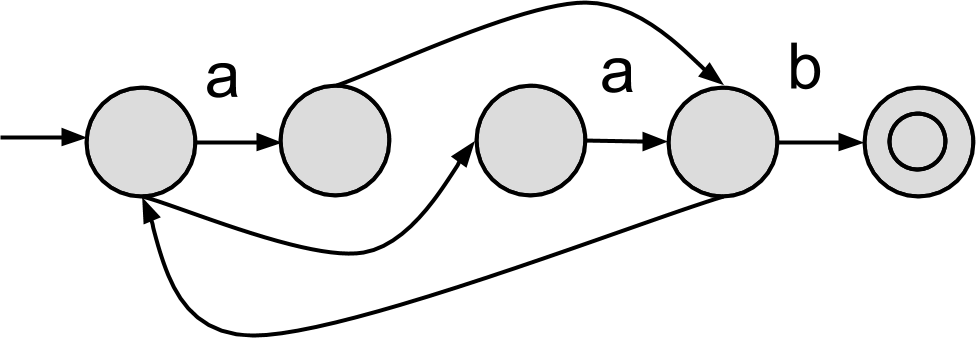
\includegraphics[scale=0.3]{figures/exemplo_automato.png}
  \caption{Exemplo de autômato para expressão regular $(a|a)+b$}
  \label{fig:exemplo_automato}
\end{figure}

Desde então, conforme as implementações foram evoluindo, muitas funcionalidades foram adicionadas à linguagem de descrição de expressões regulares que as afastaram da teoria original. Enquanto originalmente descreviam linguagens estritamente regulares, a implementação mais difundida atualmente (\emph{PCRE}) é capaz não só de reconhecer qualquer linguagem livre de contexto, como também algumas sensíveis a contexto. \cite{bib:Nikita12}

Uma das consequências mais notáveis desta evolução não planejada é que o reconhecimento de strings da linguagem, um problema com solução linear originalmente, ganhou soluções exponenciais em um grande número de implementações modernas, que inclui muitas das mais usadas. Talvez a funcionalidade mais perigosa neste sentido sejam as backreferences, que não só impedem soluções polinomiais como tornam o problema de reconhecimento NP-completo. Entretanto, mesmo nas expressões que poderiam ser reconhecidas estritamente com autômatos finitos, certas particularidades de implementação as tornam potencialmente exponenciais, no pior caso \cite{bib:Cox07}.

A Figura \ref{fig:benchmark1} mostra o crescimento no tempo de execução entre a implementação da biblioteca padrão da linguagem Python e a implementação proposta neste projeto, usando o método de Thompson. 

\begin{figure}[ht]
  \centering
  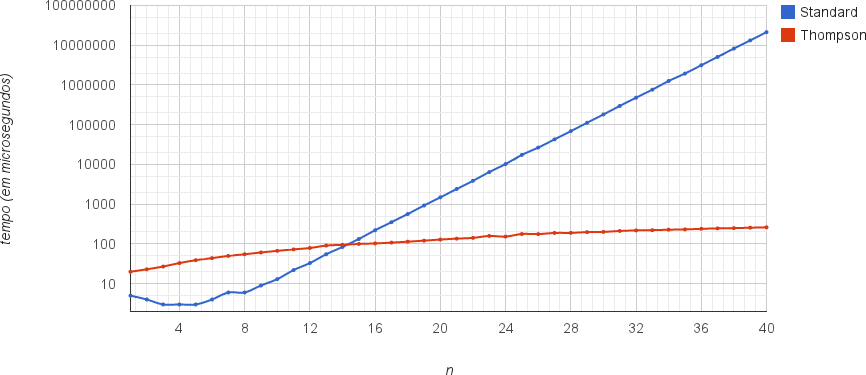
\includegraphics[scale=0.5]{figures/benchmark1.png}
  \caption{Avaliação da string $a^n$ contra a expressão $(a|a)+b$ (em escala logarítmica)}
  \label{fig:benchmark1}
\end{figure}

Essas implementações tornam o uso de expressões regulares potencialmente inseguro em situações ora triviais. Um usuário mal intencionado pode ser capaz de forçar a execução de uma expressão com caráter exponencial para efetuar um ataque de negação de serviço em um servidor web, por exemplo. 

Muitas vezes a prevenção para esse tipo de ataque pode não ser trivial, e.g. em Java, onde métodos comumente usados contra a entrada do usuário, como \emph{replaceAll} e \emph{split}, da classe \emph{String} são implementados usado expressões regulares vulneráveis a esse tipo de ataque.

Mesmo em casos onde o usuário mal intencionado não tem acesso a escrever expressões regulares, um erro de programação pode deixar o sistema vulnerável a negação de serviço. Este problema torna-se especialmente notável pelo frequente compartilhamento em repositórios online, que contém muitas expressões vulneráveis \cite{bib:Kirrage13,bib:Weidman10}. 

%~~~~~~~~~~~~~~~~~~~~~~~~~~~~~~~~~~~~~~~~~~~~~~~~~~~~~~~~~~~~~~~~~~~~~~~
\section{Objetivo}
%~~~~~~~~~~~~~~~~~~~~~~~~~~~~~~~~~~~~~~~~~~~~~~~~~~~~~~~~~~~~~~~~~~~~~~~

Este projeto tem dois objetivos principais. O primeiro é demonstrar através de testes pontuais e benchmarks os problemas fundamentais nas implementações de expressões regulares em diversas linguagens modernas, provando inclusive a NP-completude do problema de reconhecimento de strings nas linguagens que definem. O segundo objetivo é propor uma implementação didática e minimalista das expressões regulares propostas por Kleene, utilizando o método descrito por Thompson para construção e simulação do autômato. 

A implementação irá deixar de fora certas funcionalidades comuns nos \emph{sabores} mais modernos de expressão regular. Algumas destas funcionalidades podem ser implementadas sem sacrificar eficiência de execução. Outras, introduzem certa complexidade, porém mantendo a execução do algoritmo polinomial. O restante, entretanto, não é possível implementar sem tornar o algoritmo exponencial no pior caso. Todas as funcionalidades intencionalmente excluídas serão listadas e propostas de soluções serão apresentadas quando cabível.

Deseja-se mostrar com esse projeto que o problema de reconhecimento de expressões regulares pode ser resolvido de maneira eficiente, mesmo com as implementações mais simples, desde que seja observada a base teórica que as deu origem.

%~~~~~~~~~~~~~~~~~~~~~~~~~~~~~~~~~~~~~~~~~~~~~~~~~~~~~~~~~~~~~~~~~~~~~~~
\section{Estrutura}
%~~~~~~~~~~~~~~~~~~~~~~~~~~~~~~~~~~~~~~~~~~~~~~~~~~~~~~~~~~~~~~~~~~~~~~~

O projeto está divido em cinco capítulos. O capítulo 2 trata da base teórica por trás das expressões regulares, contando sua história, passando pelo método de construção do autômato de Thompson, e exibindo um algoritmo trivial (porém ineficiente) para sua solução.

O capítulo 3 descreve poder das implementações modernas de expressão regular, mostrando recursos avançados, como \emph{zero-width assertions} e \emph{backreferences}. Mostra também exemplos de expressões que reconhecem gramáticas não-regulares, exibindo o distanciamento entre estas e a teoria original. Por fim, é mostrado um benchmark comparando a performance entre as diversas implementações, que evidenciam uma diferença fundamental na forma como o problema é abordado em cada uma delas.

No capítulo 4 é proposta uma implementação de expressões regulares utilizando o método de Thompson. Os resultados teóricos e práticos desta implementação são discutidos e comparados com resultados anteriores.

O capítulo 5 expõe as conclusões e contribuições deste trabalho, bem como as dificuldades encontradas durante o projeto. Também serão listadas e descritas as funcionalidades não implementadas, possivelmente sugerindo formas eficientes de implementá-las, ou mesmo formas diferentes de simular o autômato que melhorem a eficiência geral da execução.

%======================================================================================
\chapter{Base Teórica}
%======================================================================================

%~~~~~~~~~~~~~~~~~~~~~~~~~~~~~~~~~~~~~~~~~~~~~~~~~~~~~~~~~~~~~~~~~~~~~~~
\section{Linguagens Formais}
%~~~~~~~~~~~~~~~~~~~~~~~~~~~~~~~~~~~~~~~~~~~~~~~~~~~~~~~~~~~~~~~~~~~~~~~

Linguagens formais é um tema que mistura elementos da ciência da computação, matemática e linguística. Seu papel na computação é fundamental pela relação de seus problemas com os descritos pela teoria da computação.

Uma \emph{linguagem formal} é um conjunto -- potencialmente infinito -- de \emph{palavras}, que por sua vez são combinações de elementos de um conjunto finito de símbolos chamado \emph{alfabeto}.

A operação básica entre palavras é a \emph{concatenação}. Por exemplo, se $w_1 = aaa$ e $w_2=bbb$, então $w_1w_2 = aaabbb$. Concatenação é associativa: $(w_1w_2)w_3 = w_1(w_2w_3)$; porém não comutativa: $w_1w_2 \neq w_2w_1$.

Linguagens são conjuntos, portanto a mesma notação de conjuntos é utilizada para elas. Por exemplo, $A \cup B$ representa a união de linguagens A e B, assim como $w \in A$ é uma proposição afirma que a palavra $w$ está presente na linguagem A.

É possível concatenar linguagens. Dadas linguagens $L_1$ e $L_2$,

\begin{equation*}
	L_1L_2 = \{w_1w_2 | w_1 \in L_1, w_2 \in L_2\}
\end{equation*}

E.g.: se $A = \{a, aa\}$ e $B = \{b, bb\}$, então $AB = \{ab, aab, abb, aabb\}$.


Com base na concatenação, uma operação importante em linguagens é o fecho Kleene ($L^*$), que pode ser definido como:

\begin{equation*}
	L^0 = \{\epsilon\}
\end{equation*}
\begin{equation*}
	L^i = L^{i-1}L
\end{equation*}
\begin{equation*}
	L^* = \bigcup_{i \in \mathbb{N}} L^i
\end{equation*}

E.g.: se $A = \{a, aa\}$, então $A^* = \{\epsilon, a, aa, aaa, \ldots\}$.

%~~~~~~~~~~~~~~~~~~~~~~~~~~~~~~~~~~~~~~~~~~~~~~~~~~~~~~~~~~~~~~~~~~~~~~~
\section{Gramáticas Gerativas}
%~~~~~~~~~~~~~~~~~~~~~~~~~~~~~~~~~~~~~~~~~~~~~~~~~~~~~~~~~~~~~~~~~~~~~~~

Uma das formas de representar linguagens formais é através de gramáticas gerativas. O termo ``gramática formal'' é comumente utilizado para referir-se a elas. No entanto, existem outras formas de representar gramáticas formais além deste. Este trabalho irá se limitar à definição mais comum.

Gramáticas gerativas são sistemas de reescrita, i.e. a partir de um símbolo inicial, é possível usar as regras de reescrita para produzir todas as palavras de uma linguagem. Esta operação é, de certa forma, o problema dual de reconhecer uma palavra como parte da linguagem através de um autômato \cite{bib:Ruohonen09}.

Uma gramática é formada por uma tupla $G = (N, \Sigma, P, S)$. Onde:

\begin{lcircp}
    \item N é o conjunto de símbolos não terminais. Eles não fazem parte da linguagem original, então precisam ser sempre substituídos para alcançar um símbolo válido na linguagem.
    \item $\Sigma$ é o conjunto de símbolos terminais da linguagem. Também conhecido como alfabeto.
    \item P é o conjunto de regras de produção, geralmente na forma $\alpha \rightarrow \beta$, onde $\alpha$ e $\beta$ são sequências de símbolos terminais e não-terminais.
    \item S é o símbolo inicial do sistema de reescrita. $S \in N$.
\end{lcircp}

Um exemplo de gramática é a que define expressões da forma $a^nb^n, n>0$:

\begin{equation*}
	N = \{S\}; \Sigma = \{a,b\}
\end{equation*}

\begin{equation*}
	S \rightarrow aSb
\end{equation*}
\begin{equation*}
	S \rightarrow ab
\end{equation*}

Iniciando do símbolo S, é possível começar com a regra $ab$ ou $aSb$. A primeira já forma uma palavra na linguagem que queremos descrever ($ab$), a segunda possui um símbolo não terminal. A partir dele é possível gerar as palavras na linguagem: $aabb$, $aaabbb$, etc...

Perceba que na gramática todas as regras do lado esquerdo possuem apenas um símbolo não terminal. Se fôssemos escrever uma gramática para expressões na forma $a^nb^nc^n$, precisaríamos de uma gramática mais rebuscada:

\begin{equation*}
	N = \{S, T\}; \Sigma = \{a,b,c\}
\end{equation*}


\begin{equation*}
	S \rightarrow aTSc
\end{equation*}
\begin{equation*}
	S \rightarrow abc
\end{equation*}
\begin{equation*}
	Ta \rightarrow aT
\end{equation*}
\begin{equation*}
	Tb \rightarrow bb
\end{equation*}

O fato desta gramática definir sequências de símbolos à esquerda com mais de um símbolo a torna especial. Segundo a hiearquia de Chomsky, a primeira gramática é livre de contexto, enquanto a segunda é sensível a contexto.

%~~~~~~~~~~~~~~~~~~~~~~~~~~~~~~~~~~~~~~~~~~~~~~~~~~~~~~~~~~~~~~~~~~~~~~~
\section{Hierarquia de Chomsky}
%~~~~~~~~~~~~~~~~~~~~~~~~~~~~~~~~~~~~~~~~~~~~~~~~~~~~~~~~~~~~~~~~~~~~~~~

Segundo Noam Chomsky \cite{bib:Chomsky57}, uma linguagem formal pode ser classificada em um de quatro tipos baseados na capacidade expressiva das gramáticas formais que a expressam:

\begin{lcircp}
    \item {\bf Tipo 0}: linguagens recursivamente enumeráveis (ou irrestritas)
    \item {\bf Tipo 1}: linguagens sensíveis a contexto
    \item {\bf Tipo 2}: linguagens livres de contexto
    \item {\bf Tipo 3}: linguagens regulares
\end{lcircp}

Cada conjunto é propriamente incluso no seu conjunto superior na hierarquia, como pode ser visto na Figura \ref{fig:chomsky}.

\begin{figure}[ht]
  \centering
  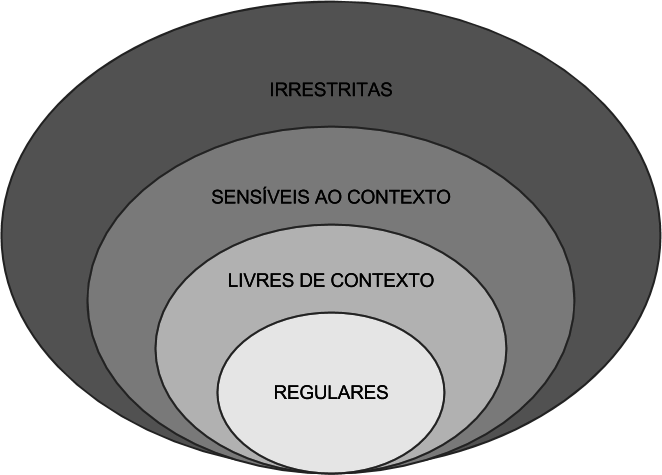
\includegraphics[scale=0.5]{figures/chomsky.png}
  \caption{Representação da inclusão de conjuntos na hiearquia de Chomsky}
  \label{fig:chomsky}
\end{figure}

\subsection{Linguagens Regulares}

Linguagens regulares são aquelas cujas regras de formação são na forma $S \rightarrow aT$ ou $S \rightarrow a$, onde \emph{S} e \emph{T} são não-terminais e \emph{a} é um terminal na linguagem. Estas linguagens são equivalentes em poder de expressão a \emph{autômatos finitos}. 

Alguns autores também incluem regras do tipo $S \rightarrow \epsilon$, desde que S não apareça do lado direito de nenhuma regra.

Exemplos de linguagens regulares incluem: endereços de email, repetição de caracteres ($a^n$), repetição independente de dois caracteres ($a^nb^m$).

\subsection{Linguagens Livres de Contexto}

Linguagens livres de contexto são linguagens onde todas as regras de formação são do tipo $S \rightarrow \gamma$, onde \emph{S} é um não-terminal e $\gamma$ é uma sequência composta por terminais e não-terminais. 

Isto na prática significa que a substituição de um não-terminal é sempre feita independente do contexto onde é encontrado. Linguagens deste tipo são equivalentes em poder expressivo a \emph{autômatos de pilha}. Elas compõem a base teórica para a maioria das linguagens de programação. 

Entre alguns exemplos clássicos de linguagens livres de contexto figuram: parênteses aninhados, repetição condicionada de dois caracteres ($a^nb^n$), expressões aritméticas.

\subsection{Linguagens Sensíveis a Contexto}
Linguagens sensíveis a contexto são linguagens onde todas as regras de formação são do tipo $\alpha S\beta\rightarrow \alpha\gamma\beta$, onde $\alpha$, $\gamma$ e $\beta$ são sequências compostas por terminais e não-terminais. Elas diferem das linguagens livres de contexto por definir -- exatamente -- contexto para que um não-terminal S seja substituído por uma sequência $\gamma$. 

Apesar de terem um escopo bem mais amplo, gramáticas deste tipo ainda são passíveis de ser computadas usando um \emph{autômato linearmente limitado}. 

Exemplos: \emph{squares} (\emph{DogDog, CatCat, WikiWiki...}), \emph{matching triplets} ($a^nb^nc^n$).

\subsection{Linguagens Recursivamente Enumeráveis}

Linguagens recursivamente enumeráveis não definem restrições para as regras de produção. Portanto, qualquer sequência de terminais e não-terminais $\alpha$ pode ser substituída por outra $\beta$. Linguagens assim são reconhecíveis por uma \emph{máquina de Turing}. 

Diferente dos tipos anteriores, quando apresentada a uma sequência que não faça parte da linguagem, não há garantia de parada da máquina, definindo o que é chamado na teoria de conjunto \emph{semi-decidível}.

Um dos exemplos mais notáveis de linguagens recursivamente enumeráveis que não são sensíveis a contexto é a sintaxe de templates do C++ \cite{bib:Veldhuizen03}.

\subsection{Tabela de Referência}

É possível resumir os tipos de linguagens da hierarquia de Chomsky numa tabela de referência quanto à máquina que a processa e os tipos de regras que aceita.

\begin{center}
	\begin{tabular}{ c | c | c | c }
		 & {\bf Linguagem} & {\bf Máquina} & {\bf Regras} \\
		\hline 
		0 & Recursivamente enumerável & Máquina de Turing 			 & 
			$\alpha \rightarrow \beta$ \\ 
		1 & Sensível a contexto 		& Autômato limitado linearmente & 
			$\alpha S\beta\rightarrow \alpha\gamma\beta$\\ 
		2 & Livre de contexto 			& Autômato de pilha 			 & 
			$S \rightarrow \gamma$\\ 
		3 & Regular 					& Autômato finito 				 &
			$S \rightarrow aT$ ou $S \rightarrow a$\\ 
	\end{tabular}
\end{center}

%~~~~~~~~~~~~~~~~~~~~~~~~~~~~~~~~~~~~~~~~~~~~~~~~~~~~~~~~~~~~~~~~~~~~~~~
\section{Expressões Regulares}
%~~~~~~~~~~~~~~~~~~~~~~~~~~~~~~~~~~~~~~~~~~~~~~~~~~~~~~~~~~~~~~~~~~~~~~~

Expressões regulares são sequências de caracteres que definem linguagens regulares. Estas sequências obedecem a algumas regras de criação. Alguns caracteres são interpretados literalmente, enquanto outros são considerados metacaracteres que controlam como os trechos da expressão se relacionam.

Por definição:

\begin{lcircp}
    \item Sequências vazias são expressões regulares.
    \item Caracteres unitários são expressões regulares. E.g. \emph{a}.
    \item Expressões regulares podem ser concatenadas para formar novas expressões. E.g. se $e_1$ reconhece \emph{a} e $e_2$ reconhece \emph{b}, então $e_1e_2$ reconhece \emph{ab}.
    \item Expressões regulares podem ser alternadas para formar novas expressões. E.g. se $e_1$ reconhece \emph{a} e $e_2$ reconhece \emph{b}, então $e_1|e_2$ reconhece \emph{a} e \emph{b}.
    \item Pode-se aplicar o fecho Kleene para formar novas expressões. E.g. se $e_1$ reconhece \emph{a}, então $e_1*$ reconhece \emph{a}, \emph{aa}, \emph{aaa}... etc., bem como string vazia.
\end{lcircp}

Perceba que é possível definir outros operadores comuns, como $?$ e $+$. Mas é possível fazê-lo a partir das operações descritas acima. O operador $e_1?$ pode ser definido como a alternância entre $e_1$ e uma string vazia. O operarador $e_1+$ pode ser definido como $e_1e_1*$.

Outros operadores sobre caracteres como o $.$ (qualquer caractere) e as classes de caractere (e.g. $[a-zA-Z]$) são trivialmente implementados usando alternação de expressões.

A precedência natural dos operadores, da mais fraca para a mais forte, é: alternância, concatenação, repetição. Assim, uma expressão como $ab|cd*$ é interpretada como exibido na Figura \ref{fig:abcd_parse_tree}.

\begin{figure}[ht]
  \centering
  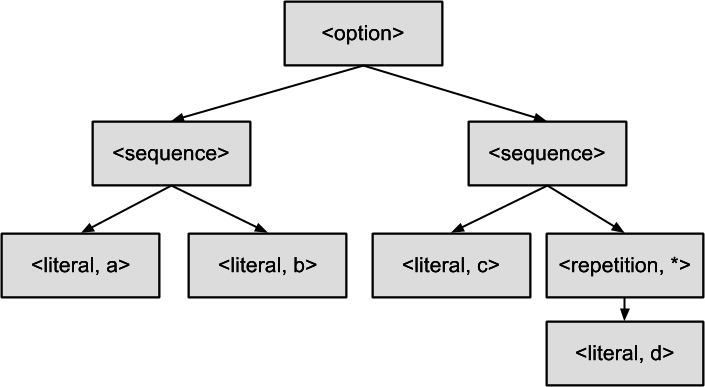
\includegraphics[scale=0.4]{figures/abcd_parse_tree.png}
  \caption{Árvore de avaliação para expressão $ab|cd*$}
  \label{fig:abcd_parse_tree}
\end{figure}

É possível agrupar sub-expressões utilizando parênteses, tal qual é feito com expressões aritméticas. Assim $a(b|c)d*$ tem um sentido completamente diferente de $ab|cd*$.

Estas operações, apesar de bastante incompletas, definem inequivocamente expressões regulares. É possível representar qualquer linguagem regular utilizando apenas estes operadores. Mais importante: é teoricamente possível reconhecer qualquer símbolo nesta linguagem com apenas uma passagem pela entrada (sem \emph{backtracking}). 

Representando apenas linguagens regulares, as expressões regulares representam um paradoxo sobre si mesmas: elas não são capazes de representar nem a própria linguagem que as define. O grande culpado disso é a presença dos parênteses agrupadores, tornando esta gramática propriamente pertencente ao conjunto das gramáticas livres de contexto.

Novas implementações de expressões regulares adicionaram novos operadores que tornam a sintaxe mais concisa. Porém, essas adições normalmente não alteram o poder expressivo das regexes. No entanto, existem adições que adicionam poder expressivo, como é o caso das \emph{backreferences}, que permitem o reconhecimento de algumas linguagens não-regulares. \emph{Backreferences} consiste em referências \emph{submatches} reconhecias anteriormente.

Por exemplo, uma linguagem composta por palavras repetidas, como \emph{DogDog} ou \emph{CatCat}. É possível definir uma expressão regular $/(.*)\backslash 1/$ que reconhece esta linguagem. o $\backslash 1$ instrui ao motor de reconhecimento a esperar uma nova palavra exatamente igual à obtido pelo reconhecimento do primeiro grupo $(.*)$.

Esta linguagem não apenas cai fora do conjunto das linguagens regulares, como também não é uma linguagem livre de contexto.

Tal poder expressivo tem seu preço. Match de backreferences é um problema NP-completo, logo, os melhores algoritmos conhecidos ainda tem pior caso exponencial. É possível, porém, escrever algoritmos polinomiais para expressões que não fazem uso de backreferences. No entanto, pela diferente natureza dos dois tipos de algoritmos, normalmente as linguagens implementam apenas um deles, fazendo com que algumas expressões que originalmente poderiam ser avaliadas em tempo polinomial serem penalizadas sem necessidade.

%~~~~~~~~~~~~~~~~~~~~~~~~~~~~~~~~~~~~~~~~~~~~~~~~~~~~~~~~~~~~~~~~~~~~~~~
\section{Autômatos Finitos}
%~~~~~~~~~~~~~~~~~~~~~~~~~~~~~~~~~~~~~~~~~~~~~~~~~~~~~~~~~~~~~~~~~~~~~~~

Autômatos finitos representam um modelo matemático de computação. Eles representam máquinas abstratas que podem se encontram em apenas um de um número finito de estados. Autômatos não possuem memória. Mas apenas estritamente falando, pois o estado atual do autômato representa sua memória. Um autômato muda de estado como reação a um estímulo externo. Formalmente, autômatos finitos são uma tupla $M = (Q, \Sigma, q_0, \delta, A)$, onde:

\begin{lcircp}
    \item Q é o conjunto de estados do autômato. Sempre finito.
    \item $\Sigma$ é o alfabeto aceito pelo autômato.
    \item $q_0$ é o estado inicial do autômato. $q_0 \in Q$.
    \item $\delta$ é a função de transição, que mapeia cada $(q_i, a) \in Q \times \Sigma$ a um subconjunto de Q. Se esse subconjunto tem apenas zero ou um elementos, o autômato é \emph{deterministico}, caso contrário, ele é \emph{não-determinístico}.
    \item A é o conjunto de estados de aceite. $A \subseteq Q$.
\end{lcircp}

Por exemplo:

\begin{figure}[ht]
  \centering
  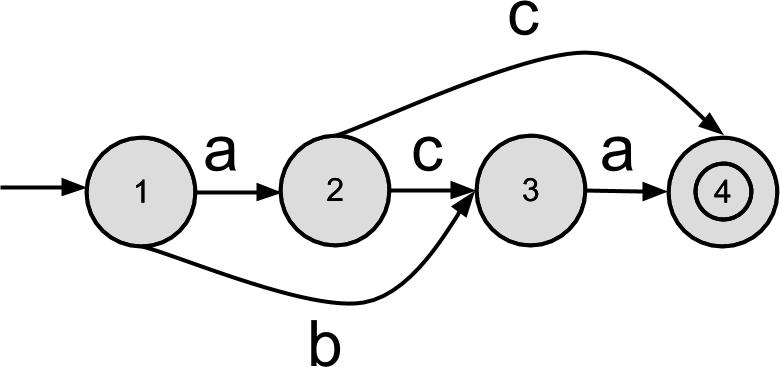
\includegraphics[scale=0.3]{figures/exemplo_automato_numerado.png}
  \caption{Diagrama de estados de um autômato não-determinístico}
  \label{fig:exemplo_automato_numerado}
\end{figure}

O autômato na Figura~\ref{fig:exemplo_automato_numerado} pode ser descrito por $M=(\{1,2,3,4\}, \{a,b,c\}, 1, \delta, \{4\})$, onde $\delta$ é definida pela tabela de transições:

\begin{center}
	\begin{tabular}{ c || c | c | c }
		{\bf $\delta$} & {\bf a} & {\bf b} & {\bf c} \\
		\hline 
		\hline 
		1 & 2 & 3 &  \\ 
		\hline 
		2 &   &   & 2, 4 \\ 
		\hline 
		3 & 4 &   &  \\ 
		\hline 
		4 &   &   &  \\ 
	\end{tabular}
\end{center}

Este autômato é \emph{não determinístico}, pois um mesmo input (c) pode gerar múltiplas transições no estado 2. Outra forma de representar autômatos não determínisticos é introduzindo a entrada $\epsilon$, como pode ser visto na Figura~\ref{fig:exemplo_automato_epsilon}. Perceba que este autômato \emph{não é equivalente} ao definido anteriormente. Ele aceita uma entrada $b$ que o primeiro não aceita.

\begin{figure}[ht]
  \centering
  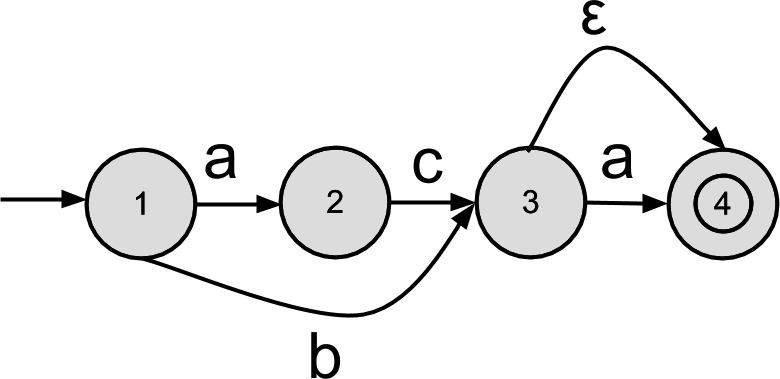
\includegraphics[scale=0.3]{figures/exemplo_automato_epsilon.png}
  \caption{Diagrama de estados de um autômato não-determinístico com entrada $\epsilon$}
  \label{fig:exemplo_automato_epsilon}
\end{figure}


Autômatos podem ser utilizados para reconhecer linguagens regulares. É possível construir um autômato que, dada uma linguagem, termina em estados de aceite ou não, dependendo da palavra que for oferecida como entrada.

O autômato descrito na Figura~\ref{fig:exemplo_automato_epsilon}, por exemplo, reconhece uma linguagem finita definida por $L = \{ac, aca, b, ba\}$. A linguagem que um autômato finito reconhece é \emph{sempre regular}. E \emph{toda linguagem regular} pode ser reconhecida com autômatos finitos \cite{bib:Kleene56}.

%~~~~~~~~~~~~~~~~~~~~~~~~~~~~~~~~~~~~~~~~~~~~~~~~~~~~~~~~~~~~~~~~~~~~~~~
\section{Método de Construção de Thompson}
%~~~~~~~~~~~~~~~~~~~~~~~~~~~~~~~~~~~~~~~~~~~~~~~~~~~~~~~~~~~~~~~~~~~~~~~

Pela equivalência entre linguagens regulares e autômatos finitos. É útil poder converter entre um e outro pela facilidade de lidar com cada um deles em situações específicas. Ken Thompson \cite{bib:Thompson68} descreveu um método para construir autômatos a partir de expressões regulares.

Na época em que foi escrito, o artigo descrevia como gerar código de máquina para um IBM 7094. Isto era necessário por restrições de hardware da época. Hoje não é mais estritamente necessário. Este trabalho irá se limitar a descrever como construir o autômato a partir da expressão regular.

Iremos assumir uma notação diferente para representação do autômato, que irá facilitar a construção. Para fins de praticidade, todo estado $q_i \in Q$ será de um entre três tipos possíveis:

\begin{lcircp}
    \item Um estado de \emph{consumo}, que possui exatamente uma transição possível dada por um caractere $a \in \Sigma$.
    \item Um estado de \emph{decisão}, que possui uma ou duas transições $\epsilon$ para estados distintos.
    \item Um estado de \emph{aceite}, que não possui qualquer transição.
\end{lcircp}

O diagrama de estados também será alterado para facilitar a visualização como pode ser visto na Figura~\ref{fig:nova_notacao}.

\begin{figure}[ht]
  \centering
  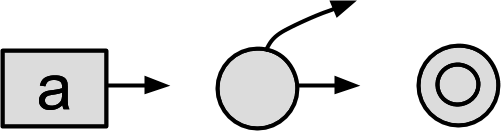
\includegraphics[scale=0.25]{figures/nova_notacao.png}
  \caption{Mesmo autômato representado com as duas notações}
  \label{fig:nova_notacao}
\end{figure}




%~~~~~~~~~~~~~~~~~~~~~~~~~~~~~~~~~~~~~~~~~~~~~~~~~~~~~~~~~~~~~~~~~~~~~~~
\section{Simulação do Autômato}
%~~~~~~~~~~~~~~~~~~~~~~~~~~~~~~~~~~~~~~~~~~~~~~~~~~~~~~~~~~~~~~~~~~~~~~~

TBD


\backmatter

\appendix

%======================================================================================
\postextualchapter{Benchmark em Python: re, pyrex}
%======================================================================================

\section{Tabela de Tempos (em microsegundos)}

\begin{center}
	\vline
	\begin{tabular}{ c || c | c }
		{\bf n} & {\bf re} & {\bf pyrex} \\
		\hline 
		1 & 5 & 20  \\ 
		2 & 4 & 23 \\ 
		3 & 3 & 27 \\ 
		4 & 3 & 33 \\ 
		5 & 3 & 39 \\ 
		6 & 4 & 44 \\ 
		7 & 6 & 50 \\ 
		8 & 6 & 55 \\ 
		9 & 9 & 61 \\ 
		10 & 13 & 67 \\ 
		11 & 22 & 73 \\ 
		12 & 33 & 79 \\ 
		13 & 55 & 91 \\ 
		14 & 84 & 95 \\ 
		15 & 133 & 100 \\ 
		16 & 221 & 103 \\ 
		17 & 353 & 108 \\ 
		18 & 566 & 114 \\ 
		19 & 927 & 121 \\ 
		20 & 1486 & 129 \\ 
	\end{tabular}
	\vline
	\quad
	\vline
	\begin{tabular}{ c || c | c }
		{\bf n} & {\bf re} & {\bf pyrex} \\
		\hline 
		21 & 2409 & 136 \\ 
		22 & 3875 & 142 \\ 
		23 & 6438 & 159 \\ 
		24 & 10251 & 153 \\ 
		25 & 17418 & 178 \\ 
		26 & 26590 & 177 \\ 
		27 & 42723 & 189 \\ 
		28 & 68890 & 190 \\ 
		29 & 111910 & 198 \\ 
		30 & 181338 & 201 \\ 
		31 & 296340 & 212 \\ 
		32 & 478507 & 219 \\ 
		33 & 763335 & 222 \\ 
		34 & 1259066 & 228 \\ 
		35 & 1937591 & 232 \\ 
		36 & 3136469 & 240 \\ 
		37 & 5078676 & 246 \\ 
		38 & 8261930 & 250 \\ 
		39 & 13229837 & 256 \\ 
		40 & 21334059 & 262 \\
	\end{tabular}
	\vline
\end{center}

\newpage
\section{Gráfico}

\begin{figure}[ht]
  \centering
  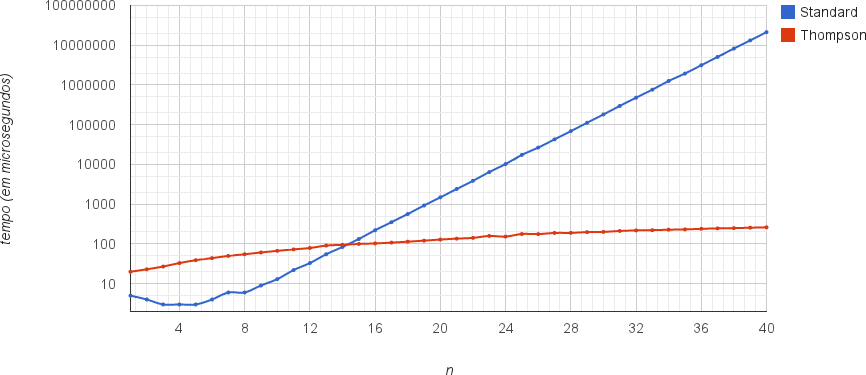
\includegraphics[scale=0.5]{figures/benchmark1.png}
\end{figure}

\section{Código fonte}

\begin{verbatim}
import re, pyrex

from timeit import timeit

r1 = re.compile('(a?a)+b')
r2 = pyrex.rex('(a?a)+b')

def time(r, i):
    return timeit(lambda: r.match('a'*i), number=1)*1e6

for i in xrange(1, 41):
    print '{}\t{:8.0f}\t{:8.0f}'.format(
        i, time(r1, i), time(r2, i))
\end{verbatim}

\bibliography{bibliografia}

\end{document}

